\documentclass{article}

\usepackage{graphicx}
\usepackage{tikz}
\usepackage{tikzsymbols}
\usetikzlibrary{calc,patterns,shapes.geometric}
\pagestyle{empty}
\usepackage[margin=0pt]{geometry}
\geometry{papersize={14in,12in}}

\def\centerarc[#1](#2)(#3:#4:#5){\draw[#1] ($(#2)+({#5*cos(#3)},{#5*sin(#3)})$) arc (#3:#4:#5);}

\begin{document}
	\begin{figure}
		\centering
		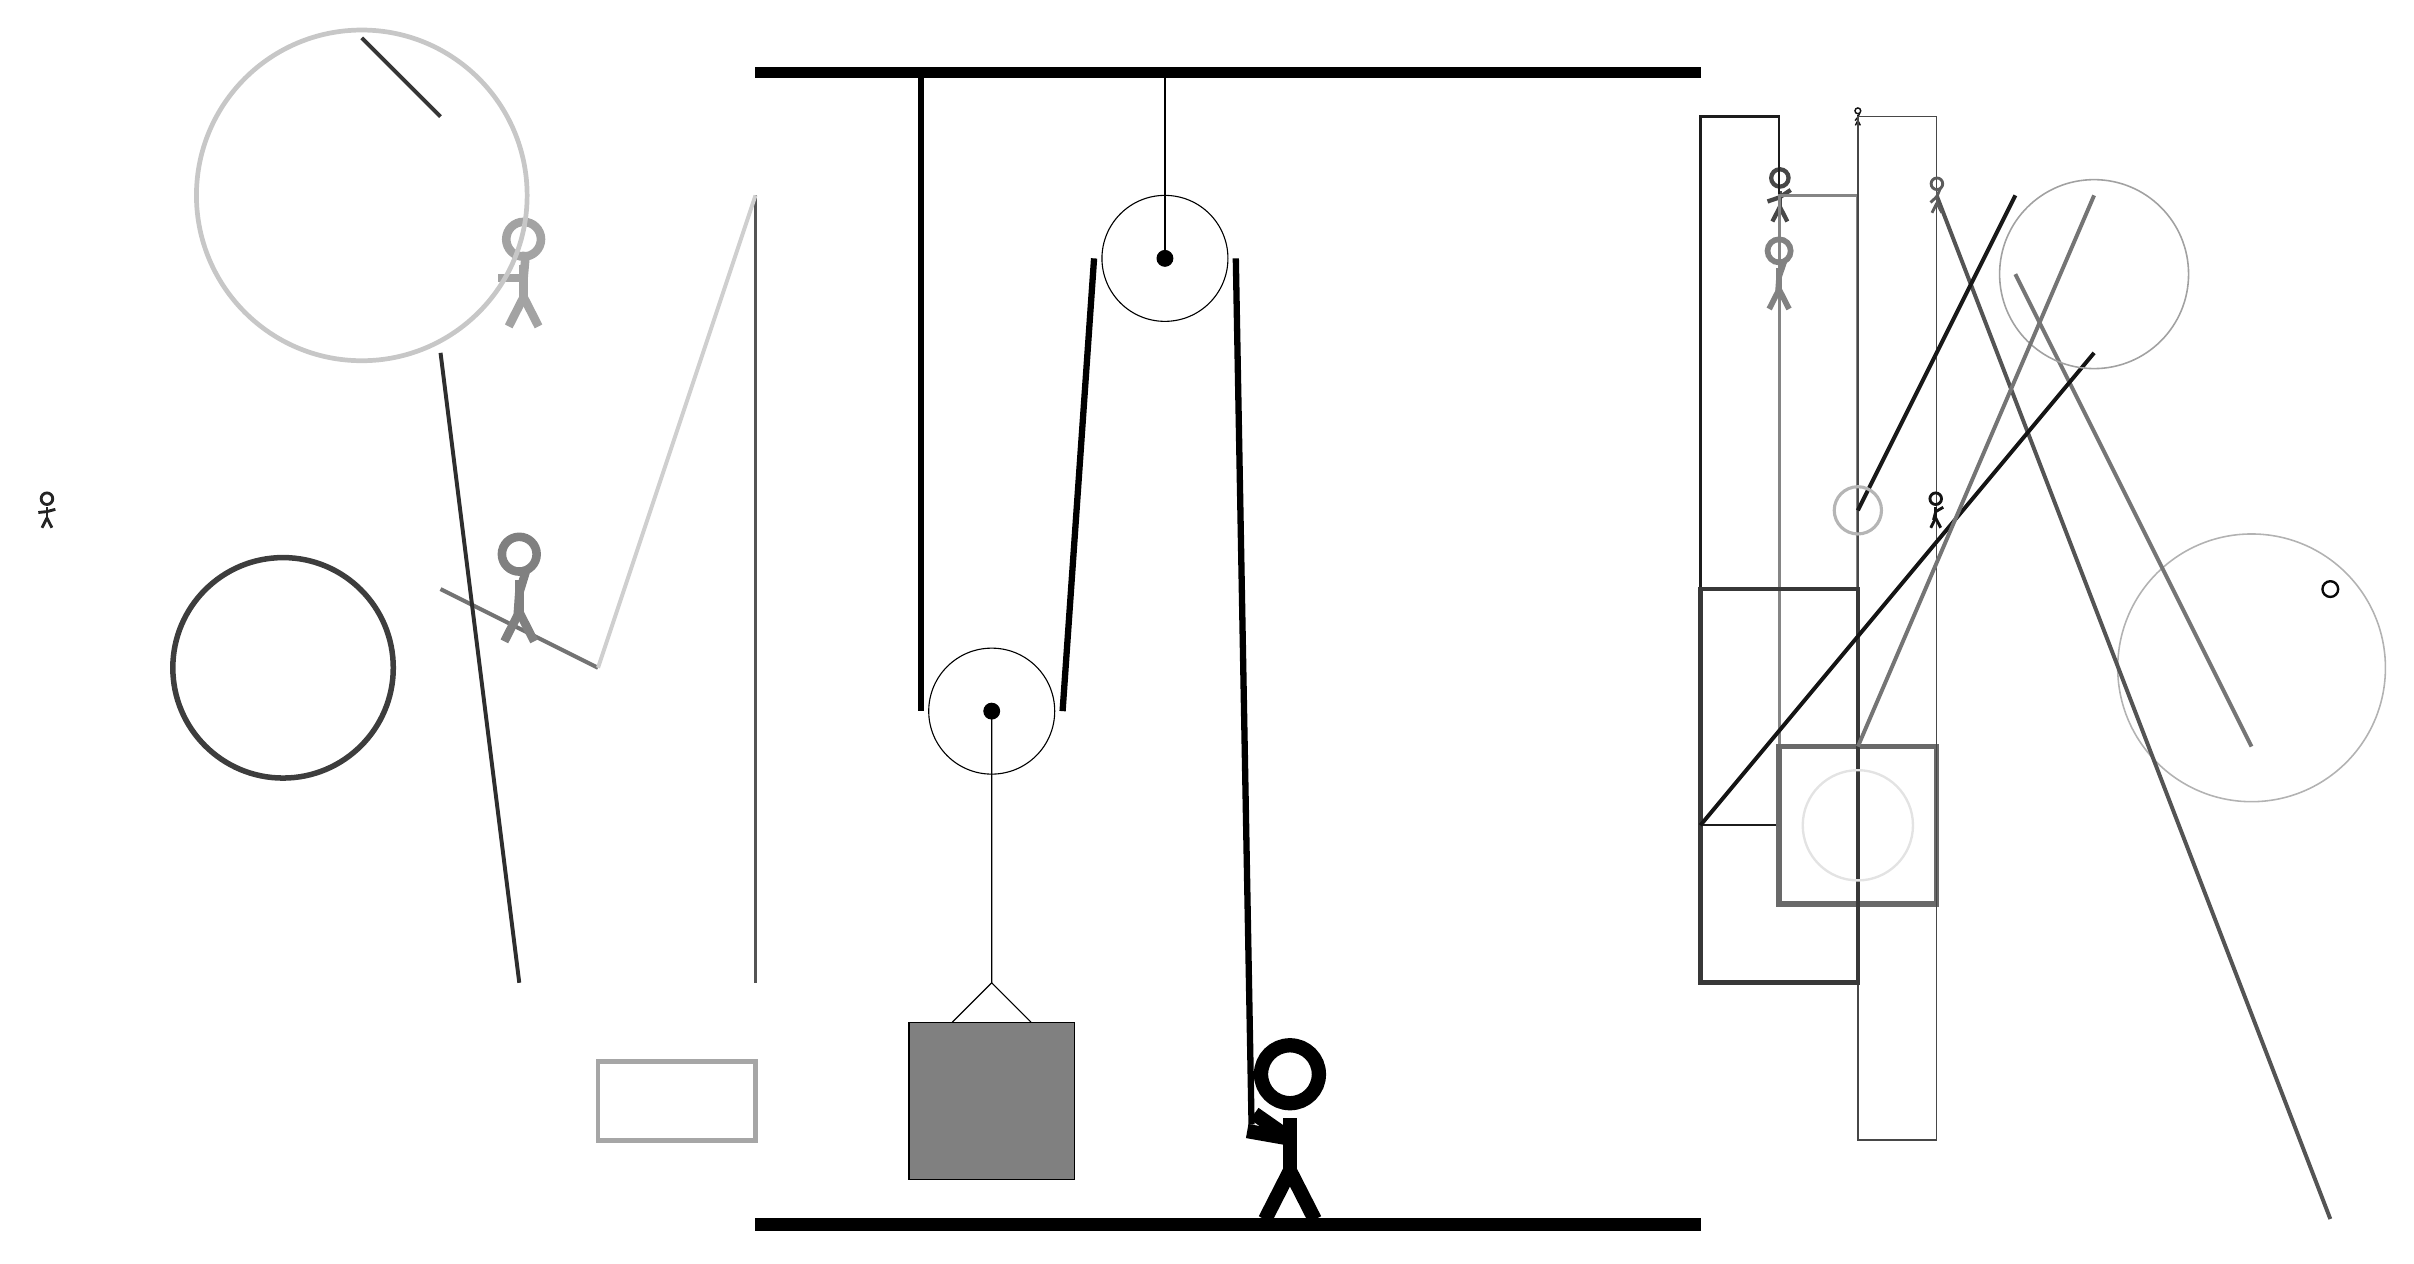
\begin{tikzpicture}
			%%%%% START %%%%%
			
			\draw[fill=black] (-2, 11.5) rectangle (10, 11.625);
			
			\node[line width=0.2mm, color=black!72] at (11, 10) {\Strichmaxerl[3][19][34]};
			
			\draw[line width=0.3mm, color=black!89] (10, 11) rectangle (11, 2);
			\draw[line width=0.4mm, color=black!48] (11, 1) rectangle (12, 10);
			\draw [line width=0.2mm, color=black!30](17, 4) circle (1.7);
			
			\draw[line width=0.5mm, color=black!79](-6, 11) -- (-7, 12);
			\draw[line width=0.5mm, color=black!54](14, 9) -- (17, 3);
			\node[line width=0.4mm, color=black!36] at (-5, 9) {\Strichmaxerl[6][0][85]};
			\node[line width=0.4mm, color=black!86] at (-11, 6) {\Strichmaxerl[2][6][15]};
			\node[line width=0.2mm, color=black!93] at (12, 11) {\Strichmaxerl[1][50][66]};
			\draw[line width=0.6mm, color=black!35] (-4, -1) rectangle (-2, -2);
			\draw[line width=0.7mm, color=black!59] (11, 1) rectangle (13, 3);
			\draw[line width=0.5mm, color=black!67] (-2, 0) rectangle (-2, 10);
			\draw[line width=0.2mm, color=black!72] (12, 11) rectangle (13, -2);
			
			\draw[line width=0.5mm, color=black!67](13, 10) -- (18, -3);
			\draw[line width=0.5mm, color=black!55](-6, 5) -- (-4, 4);
			\draw[line width=0.5mm, color=black!90](14, 10) -- (12, 6);
			
			\node[line width=0.2mm, color=black!92] at (13, 6) {\Strichmaxerl[2][75][30]};
			\draw[line width=0.5mm, color=black!19](-2, 10) -- (-4, 4);
			\draw[line width=0.6mm, color=black!78] (10, 5) rectangle (12, 0);
			\node[line width=0.5mm, color=black!49] at (11, 9) {\Strichmaxerl[4][86][71]};
			\node[line width=0.4mm, color=black!50] at (-5, 5) {\Strichmaxerl[6][86][73]};
			
			\draw [line width=0.3mm, color=black!11](12, 2) circle (0.7);
			
			\draw[line width=0.5mm, color=black!92](10, 2) -- (15, 8);
			\draw[line width=0.5mm, color=black!82](-6, 8) -- (-5, 0);
			\node[line width=0.2mm, color=black!64] at (13, 10) {\Strichmaxerl[2][42][68]};
			
			\draw [line width=0.6mm, color=black!22](-7, 10) circle (2.1);
			\draw [line width=0.7mm, color=black!76](-8, 4) circle (1.4);
			\draw [line width=0.4mm, color=black!29](12, 6) circle (0.3);
			\draw [line width=0.2mm, color=black!37](15, 9) circle (1.2);
			
			\draw[line width=0.5mm, color=black!54](12, 3) -- (15, 10);
			\draw [line width=0.3mm, color=black!97](18, 5) circle (0.1);
			
			\draw (3.2, 9.2) circle (0.8);
			\draw[fill=black] (3.2, 9.2) circle (0.1);
			\draw[thick] (3.2, 9.2) -- (3.2, 11.5);
			
			\draw (1, 3.45) circle (0.8);
			\draw[fill=black] (1, 3.45) circle (0.1);
			
			\draw (1, 3.45) -- (1, 0.0) -- (0.5, -0.5);
			\draw (1, 0.0) -- (1.5, -0.5);
			\draw[fill=black!50] (-0.05, -0.5) rectangle (2.05, -2.5);
			
			\draw[line width=0.8mm] (0.1, 11.5) -- (0.1, 3.45);
			\centerarc[line width=0.8mm](1, 3.45)(180:360:0.9);
			\draw[line width=0.8mm](1.9, 3.45) -- (2.3, 9.2);
			\centerarc[line width=0.8mm](3.2, 9.2)(0:180:0.9);
			\draw[line width=0.8mm](4.1, 9.2) -- (4.3, -1.8);
			
			\node at (4.7, -1.9) {\Strichmaxerl[10][-35][170]};
			
			\draw[fill=black] (-2, -3) rectangle (10, -3.15);
			
			%%%%% END %%%%%
		\end{tikzpicture}
	\end{figure}	
\end{document}